\documentclass{article}

% if you need to pass options to natbib, use, e.g.:
     \PassOptionsToPackage{numbers, compress}{natbib}

\usepackage[preprint]{notes}


\newcommand{\ignore}[1]{}
% to avoid loading the natbib package, add option nonatbib:
\usepackage{dsfont}
\input{preamble}
\usepackage{tikz}
\usetikzlibrary{shapes.geometric, arrows}
%  \usepackage{subfigure} 
\pdfminorversion=7

%\floatname{algorithm}{Procedure}
\renewcommand{\algorithmicrequire}{\textbf{Input:}}
\renewcommand{\algorithmicensure}{\textbf{Output:}}
\newcommand{\bsl}[1]{\boldsymbol{#1}}
\newcommand{\one}[1]{\norm{#1}_{1}}
\newcommand{\bfs}[1]{\textbf{({#1}) }}
\newcommand{\typss}{\mathcal{P}_n}

\usepackage[utf8]{inputenc} % allow utf-8 input
\usepackage{microtype}      % microtypography

%\tikzstyle{input} = [rectangle, rounded corners, minimum width=1cm, minimum height=1cm,text centered, draw=black]
%\tikzstyle{process} = [rectangle, minimum width=3cm, minimum height=1cm, text centered, draw=black]
%\tikzstyle{output} = [rectangle, rounded corners, minimum width=1cm, minimum height=1cm,text centered, draw=black]
\title{Models of Random Graphs}

\usepackage{titlesec}

\setcounter{secnumdepth}{4}

\titleformat{\paragraph}
{\normalfont\normalsize\bfseries}{\theparagraph}{1em}{}
\titlespacing*{\paragraph}
{0pt}{3.25ex plus 1ex minus .2ex}{1.5ex plus .2ex}

\begin{document}

\maketitle
\section{Notation}
\subsection{Graph}
All graphs are simple and undirected, unless otherwise stated. We use standard notation for graphs. 
\begin{defa}{\bfs{Vertex, Edges, Size}}
\begin{itemize}
    \item $V(G)$ is the \tb{vertex set} of a graph $G$, $v_{G}=|V(G)|$ is the number of vertices (sometimes write as $v(G)$)
    \item   $E(G)$ is the \tb{edge set}, $e_{G}=|E(G)|$ is the number of edges  (sometimes write as $e(G)$)
    \item In this note the \tb{size} of $G$ always means $v(G)$. We also call $v(G)$ the \tb{order} of $G$.
\end{itemize}
\end{defa}
\begin{defa}{\bfs{Density,  Maximum Density}}
\begin{itemize}
    \item Let $d(G)=e_{G} / v_{G}$ be the \tb{density} of $G$.
    \item $m(G)=\max _{H \subseteq G} d(H)$ the \tb{maximum density} of $G$. 
    \item  \tb{relative density of $G$}: another measure of the density of a graph $G$, ranging between 0 and 1, defined as $\rho(G)=e(G) /\binom{v(G)}{2}.$
\end{itemize}
\begin{rema}
Note that $d(G)$ equals half the average degree of $G$
\end{rema}
\end{defa}
\begin{defa}{\bfs{minimum, maximum degree, chromatic, degeneracy, stability number}}
\begin{itemize}
    \item $\delta(G)$ is the minimum degree,
    \item  $\Delta(G)$ is the maximum degree, 
    \item $\chi(G)$ is the chromatic number: minimum number of color
    \item $D(G)=\max _{H \subseteq G} \delta(H)$ is the degeneracy number,
    \item  $\alpha(G)$ is the stability number (the size of the largest stable, or independent, set of vertices)
    \item   $\operatorname{aut}(G)$ is the number of automorphisms of $G$.
\end{itemize}
\end{defa}
\begin{defa}{\bfs{Neighborhood}}
\begin{itemize}
    \item  We let $N(v)=N_{G}(v)$ denote the neighborhood of a vertex $v$ in $G$, that
is, the set $\{w \in V(G): v w \in E(G)\} .$ Its size is called the degree of $v$ and is denoted by $\operatorname{deg}(v)=\operatorname{deg}_{G}(v)$. 
\item  Similarly, if $S \subseteq V(G)$, its neighborhood $N_{G}(S)=\bigcup_{v \in S} N_{G}(v) \backslash S$ is the set of all vertices outside $S$ adjacent to at least one vertex in $S .$
\item Moreover, we let $\bar{N}_{G}(v)=N_{G}(v) \cup\{v\}$ and $\bar{N}_{G}(S)=$ $N_{G}(S) \cup S$ denote the corresponding closed neighborhoods, which include $v$ and $S$, respectively.
\end{itemize}
\end{defa}

\begin{defa}{\bfs{null and empty}}
 \begin{itemize}
     \item Any graph without edges will be called \tb{empty},
     \item The graph with no vertices (and thus no edges) will be called the \tb{null} graph and denoted by $\emptyset .$
 \end{itemize} 
\end{defa}
\begin{exma}{\bfs{some examples}}

\begin{enumerate}
    \item the complete graph $K_{n}$ on $n$ vertices
    \item the complete bipartite graph $K_{m, n}$ on $m+n$ vertices
    \item the cycle $C_{k}$ with $k$ vertices
    \item the path $P_{k}$ with $k$ edges and thus $k+1$ vertices
    \item the star is any graph $K_{1, n}, n \geq 0$
\end{enumerate}

\end{exma}

\begin{defa}{\bfs{Matching and Vertex-Disjoint Copies}}
 We let $j G$ denote the union of $j$ vertex-disjoint copies of $G .$ A matching is a forest consisting of isolated edges only (i.e., a graph of the form $\left.j K_{2}, j \geq 0\right)$. 
\end{defa}
\begin{defa}{\bfs{Subgraph}}
\begin{enumerate}
    \item \tb{subgraph by vertex}: If $G$ is a graph and $V \subseteq V(G)$, then $G[V]$ denotes the restriction of $G$ to $V$, defined as the graph with vertex set $V$ and edge set $E(G) \cap[V]^{2} ;$ 
    \item \tb{subgraph by edge}:  If $E \subseteq[V(G)]^{2}, G[E]$ denotes the graph with vertex set $V(G)$ and edge set $E(G) \cap E .$ 
\end{enumerate}
 A subgraph of $G$ of the type $G[V]$ is called \tb{induced or spanned} by $V$, while a subgraph of the type $G[E]$ is called \tb{spanning}. 
\end{defa}
\begin{rema}{\bfs{notation clarify}}
The number of edges in the subgraph $G[V]$ is sometimes denoted by $e_{G}(V)=e(V)$, while for two disjoint subsets $A, B \subset V(G)$, the quantity $e_{G}(A, B)$ counts the number of edges of $G$ with one endpoint in $A$ and the other in $B$.
\end{rema}
\begin{rema}{\bfs{copy vs. induced copy}}
\begin{itemize}
    \item a copy of a given graph $G$ inside another graph $F$:  any (not necessarily induced) subgraph of $F$ which is \tb{isomorphic} to $G .$
    \item an induced copy of $G$:  the above isomorphic subgraph happens to be induced.
\end{itemize}
\end{rema}
Although we define our random graphs as labelled, we are mainly interested in properties that are independent of the labelling, that is, properties that depend on the isomorphism type only. Such properties are called \tb{graph properties}.

\subsection{Asymptotics}
\begin{figure}[ht]
 \centering
 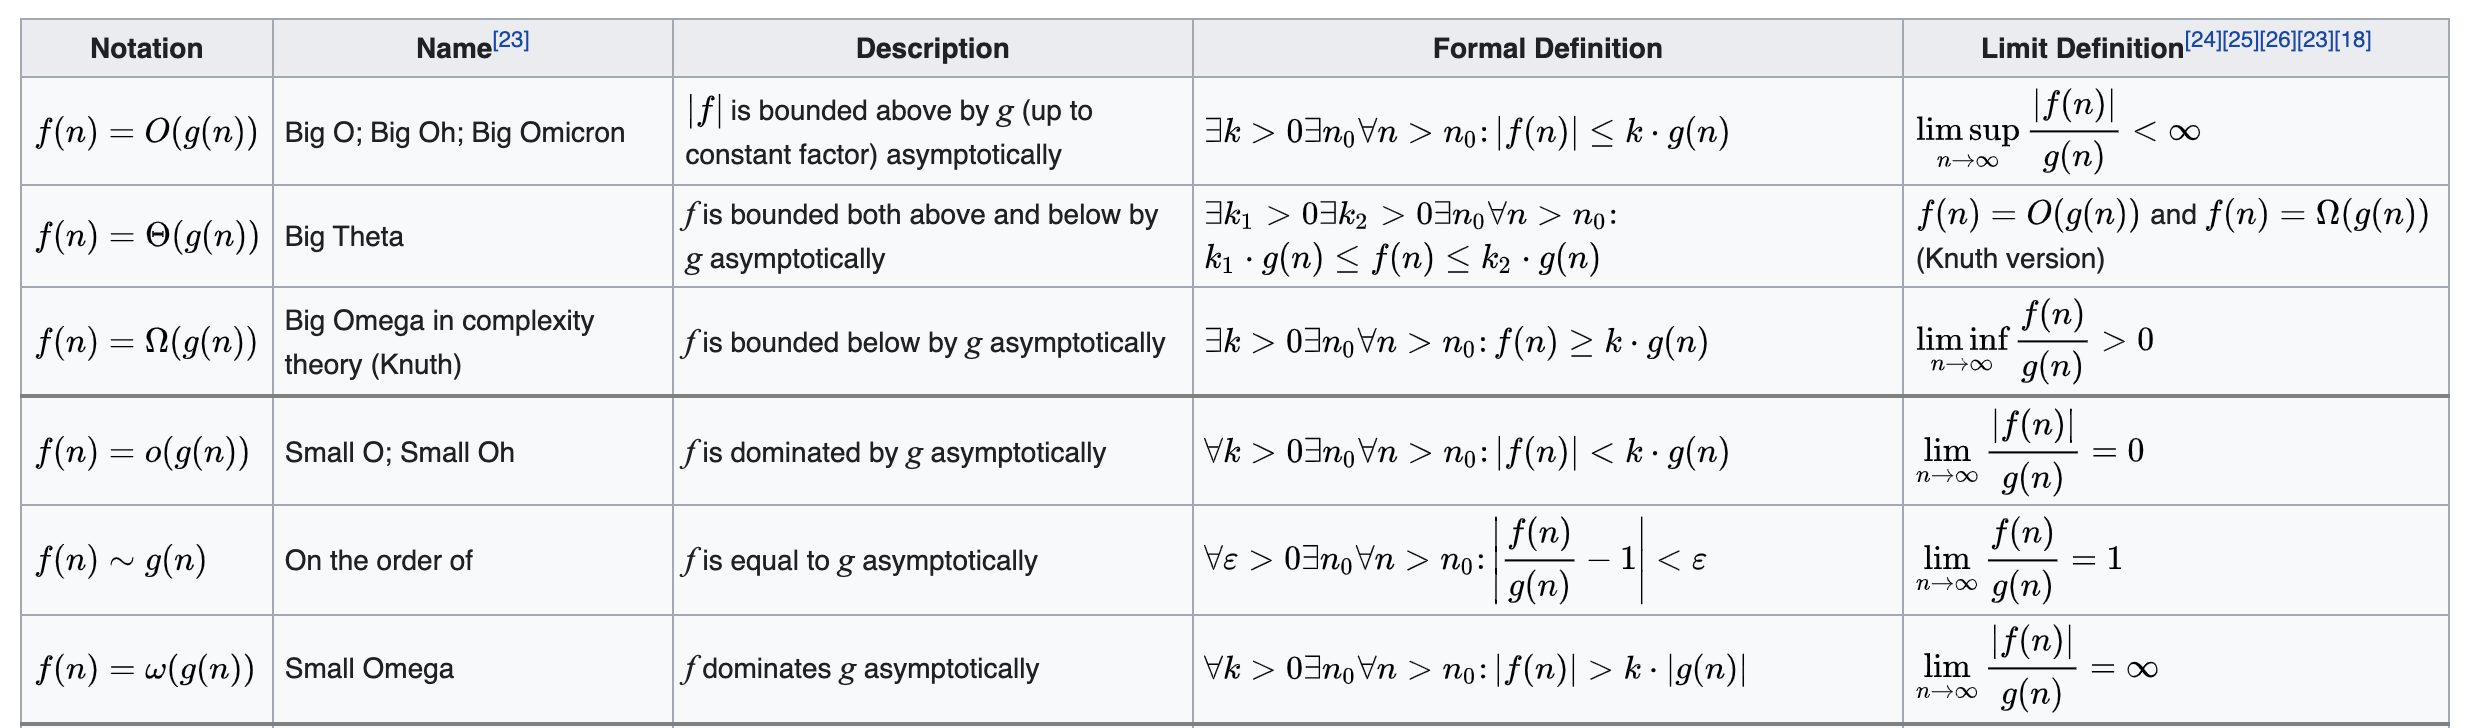
\includegraphics[width=1\linewidth]{Figs/big_o.png}
\centering
\caption{Big O notation}
		\label{un:figbigo}
\end{figure}
We may also write the following in this note:
\begin{enumerate}
    \item $a_{n} \asymp b_{n}$ if $a_{n}=\Theta\left(b_{n}\right)$
    \item $a_{n} \ll b_{n}$ or $b_{n} \gg a_{n}$ if $a_{n} \geq 0$ and $a_{n}=o\left(b_{n}\right)$
\end{enumerate}

\subsection{Probability Asymptotics}
\begin{defa}{\bfs{Asymptotically Almost Surely of Events}}
 We say that an event $E _{n}$, describing a property of a random structure depending on a parameter $n$, holds \tb{asymptotically almost surely (abbreviated a.a.s.),} if $$\P \left( E _{n}\right) \rightarrow 1 \text{ as } n \rightarrow \infty$$
\end{defa}
\begin{rema}
It is not the same as the a.s. 
\end{rema}
\begin{defa}{\bfs{Asymptotics of Random Variables}} When discussing asymptotics of random variables, we avoid expressions like $" X_{n}=O(1)$ a.a.s." or " $X_{n}=o(1)$ a.a.s.", which may be ambiguous, since they combine two asymptotic notions. Let $X_{n}$ be random variables and $a_{n}$ positive real numbers. We then define:
 \begin{enumerate}
     \item $X_{n}=O_{p}\left(a_{n}\right)$ as $n \rightarrow \infty$ if for every $\delta>0$ there exist constants $C_{\delta}$ and $n_{0}$ such that $\P \left(\left|X_{n}\right| \leq C_{\delta} a_{n}\right)>1-\delta$ for every $n \geq n_{0}$
     \item $X_{n}=O_{C}\left(a_{n}\right)$ as $n \rightarrow \infty$ if there exists a constant $C$ such that a.a.s. $\left|X_{n}\right| \leq C a_{n}$
     \item $X_{n}=\Theta_{p}\left(a_{n}\right)$ as $n \rightarrow \infty$ if for every $\delta>0$ there exist constants $c_{\delta}>0$ $C_{\delta}>0$ and $n_{0}$ such that $\P \left(c_{\delta} a_{n} \leq X_{n} \leq C_{\delta} a_{n}\right)>1-\delta$ for every $n \geq n_{0}$.
     \item $X_{n}=\Theta_{C}\left(a_{n}\right)$ as $n \rightarrow \infty$ if there exist positive constants $c$ and $C$ such that a.a.s. $c a_{n} \leq X_{n} \leq C a_{n} .$
     \item $X_{n}=o_{p}\left(a_{n}\right)$ as $n \rightarrow \infty$ if for every $\varepsilon>0$, a.a.s. $\left|X_{n}\right|<\varepsilon a_{n}$.
 \end{enumerate}
\end{defa}

\begin{rema}{\bfs{relations}}
\begin{enumerate}
    \item $X_{n}=O_{C}\left(a_{n}\right)$ implies $X_{n}=O_{p}\left(a_{n}\right)$, but not conversely. For example, any sequence $X_{n}$ of identically distributed random variables is $O_{p}(1)$, but such a sequence is $O_{C}(1)$ only if the common distribution has support in a finite interval.
    \item $X_{n}=O_{C}\left(a_{n}\right)$ if and only if the constant $C_{\delta}$ in the definition of $O_{p}$ can be chosen independently of $\delta$.
    \item $X_{n}=\Theta_{C}\left(a_{n}\right)$ implies $X_{n}=\Theta_{p}\left(a_{n}\right)$, but not conversely.
    \item $X_{n}=o_{p}\left(a_{n}\right)$ implies $X_{n}=O_{C}\left(a_{n}\right)$, and of course $X_{n}=O_{p}\left(a_{n}\right)$ 
\end{enumerate}
\end{rema}
\begin{rema}{\bfs{alternative form 1}}\label{rema:alt}
\begin{enumerate}
    \item $X_{n}=O_{p}\left(a_{n}\right)$ if and only if for 
    \tb{every} function $\omega(n) \rightarrow \infty,\left|X_{n}\right| \leq \omega(n) a_{n}$ a.a.s.
    
    ``$\Rightarrow$'' Assume $\exists \omega(n) \rightarrow \infty,$ s.t. we could get $\P(\left|X_{n_j}\right| < \omega(n_j) a_{n_j})<1-\epsilon$ for one $\epsilon>0$ and one subsequence $\{n_j\}$. Let $\delta=\epsilon$, for any $C_{\delta}$, for any $n_{0}$, we can have one $n_j>n_0$ with $\omega(n_j)>C_{\delta}$ (because of $\omega(n)$)  s.t. $\P \left(\left|X_{n_j}\right| \leq  C_{\delta} a_{n_j}\right)<\P \left(\left|X_{n_j}\right| \leq \omega(n_j) a_{n_j}\right)<1-\delta$.\\
    ``$\Leftarrow$'' Assume $X_{n}\ne O_{p}\left(a_{n}\right)$. We can find one $\delta$ so that for an increasing unbounded sequence $C_{\delta,1}<C_{\delta,2}<\ldots$, $\exists$ subsequence $\{n_i\}$ so that $\P \left(\left|X_{n_i}\right| \leq C_{\delta,i} a_{n_i}\right)<1-\delta$. Let $\omega(n)$ be $C_{\delta,i}$. We get the conclusion.
    
    \item  $X_{n}=o_{p}\left(a_{n}\right)$ if and only if for \tb{some} function $\omega(n) \rightarrow \infty,\left|X_{n}\right| \leq a_{n} / \omega(n)$ a.a.s.
    
    We only need to note the relation between $\frac{1}{\omega(n)}$ and the arbitrary small $\epsilon$:\\
    ``$\Rightarrow$'' We can find two decreasing (to $0$ ) sequences $\{\epsilon_i\}$ and $\{\delta_i\}$, such that $\P(\frac{X_n}{a_n}<\epsilon_i)>1-\delta_i$ for all $n>n_i$, where $\{n_i\}$ is a subsequence. We then define $\omega(n)$ to be $\ofrac{\epsilon_i}$ for $n_i<n\le n_{i+1}$.\\
     ``$\Leftarrow$'' For any $\epsilon$, we can have get $n_0$ such that $\frac{1}{\omega(n)}<\epsilon$ for $n>n_0$. We then have $\P(\frac{X_n}{a_n}<\epsilon)>\P(\frac{X_n}{a_n}<\frac{1}{\omega(n)})>1-\delta$ for all $n>\max\{n_0,n_1\}$, where for $\delta$ we select $n_1$ such that  $\P(\frac{X_n}{a_n}<\frac{1}{\omega(n)})>1-\delta$ for $n>n_1$.
     
     \item $X_{n}=\Theta_{p}\left(a_{n}\right)$ if and only if for 
    \tb{every} function $\omega(n) \rightarrow \infty,X_{n} \leq \omega(n) a_{n}$ a.a.s. and $X_{n}\geq a_{n}/\omega(n) $ a.a.s.
    
    We only need to additionally prove ``for every $\delta>0$ there exist constants $c_{\delta}$ and $n_{0}$ such that $\P \left(X_{n} \geq c_{\delta} a_{n}\right)>1-\delta$ for every $n \geq n_{0}$'' $\Leftrightarrow$ ``for every function $\omega(n) \rightarrow \infty,X_{n}\geq a_{n}/\omega(n) $ a.a.s.'' This is similar to 1. and we omit the details here.
    
\end{enumerate}
\end{rema}

\begin{rema}{\bfs{alternative form 1}}
\begin{enumerate}
    \item $X_{n}=o_{p}\left(a_{n}\right)$ if and only if $X_{n} / a_{n} \stackrel{p}{\rightarrow} 0 .$ (note it's the form $\P(|\frac{X_n}{a_n}|<\epsilon)$)
    \item $X_{n} \stackrel{p}{\rightarrow} a$ if and only if $X_{n}=$
$a+o_{p}(1)$
\item $X_{n} \stackrel{p}{\rightarrow} Y$ if and only if $X_{n}=Y+o_{p}(1)$
\end{enumerate}
\end{rema}
\begin{rema}
The symbol $O_{p}$ can also be expressed by equivalent standard probabilistic concepts. In fact, a sequence $X_{n}$ is bounded in probability, or tight, if $X_{n}=O_{p}(1) .$ Hence, 
$$X_{n}=O_{p}\left(a_{n}\right)\text{$\Longleftrightarrow$ if the sequence }X_{n} / a_{n}\text{ is bounded in probability (or tight).}$$
\end{rema} 

The base of all logarithms is $e$, unless specified otherwise.

\section{Introduction of Random Graphs}
\begin{defa}{\bfs{Erd\"{o}s Random Graph}}\label{deferdos}
The probability space is $(\Omega, \calF , \P )$, where $\Omega$ is the set of all graphs with vertex set $[n]\coloneqq\{1,\ldots,n\}$, $\calF$ is the family of all subsets of $\Omega$, and for every $\omega \in \Omega$.
\begin{align*}
\P (\omega)=2^{-\binom{n}{2}}
\end{align*}
\end{defa}
\begin{rema}
This probability space can also be viewed as the product of $\left(\begin{array}{l}n \\ 2\end{array}\right)$ binary spaces. In simple words, it is a result of $\binom{n}{2}$ \tb{independent} tosses of a fair coin, where "turning up heads" means "drawing an edge".
\end{rema}
\begin{defa}{\bfs{General Definition of Random Graph}}\label{def:gera}
A random graph is a graph constructed by a random procedure. In accordance with standard definitions in probability theory, this is formalized by representing the "random procedure" by a probability space $(\Omega, \calF , \P )$ and the "construction" by a function from the probability space into a suitable family of graphs. The distribution of a random graph is the \tb{induced probability distribution} on the family of graphs;
\end{defa}  
\begin{rema}
For many purposes we usually care only the distribution and do not distinguish between different random graphs with the same distribution (just like the entropy). However, please note that it is not sufficient to formally define a random graph as a probability distribution only, an important case in which this would not do is when several random graphs are considered at once, for example, in the two-round exposure described at the end of this section.
\end{rema} 
\begin{rema}
The whole theory of random graphs is  asymptotic in its nature.
\end{rema}
\subsection{Two Basic Models}
Among several models of random graphs, there are two basic ones, the binomial model and the uniform model. Both fall into the framework of random subsets of a set (see \cref{subsecransub} for details).
\subsubsection{Binomial Random Graph with Independent Edge Presence}
\begin{defa}{\bfs{Binomial Random Graph $G (n, p)$}}
Given a real number $p, 0 \leq p \leq 1$, the \tb{binomial random graph}, denoted by $G (n, p)$, is defined by taking as $\Omega$ the set of all graphs on vertex set $[n]$ and setting
\begin{align*}
\P (G)=p^{e_G}(1-p)^{\binom{n}{2})-e_G}
\end{align*}
where $e_{G}=|E(G)|$ stands for the number of edges of $G .$ It can be viewed as a result of $\binom{n}{2}$ independent coin flippings, one for each pair of vertices, with the probability of success (i.e., drawing an edge) equal to $p$. 
\end{defa}
\begin{rema}
For $p=1 / 2$ this is the model \cref{deferdos}. However, most of the random graph literature is devoted to cases in which $p=p(n) \rightarrow 0$ as $n \rightarrow \infty$. Binomial models are sometimes called Bernoulli.
\end{rema}

The binomial model is a special case of a reliability network. 

\begin{defa}{\bfs{Reliability Network: extension of $G (n, p)$}}
Let $\Omega$ is the family of all spanning subgraphs of a given graph $F$ and $\P (G)=p^{e_G}(1-p)^{e_{F}-e_{G}}$. (By a spanning subgraph we mean a graph $G$ such that $V(G)=V(F)$ and $E(G) \subseteq E(F) .$) Thus, in a reliability network, the edges of a given graph (network) are independently destroyed, each with failure probability $1-p$.
\end{defa}
\begin{rema}
One can generalize this model even further, by allowing different probabilities of failure at different edges. 
\end{rema}
\begin{rema}{\bfs{special cases}}
Taking $F=K_{n}$, the complete graph on $n$ vertices, we obtain the model $G (n, p) .$ Taking $F=K_{m, n}$, the complete bipartite graph (here either $m$ is a function of $n$, or they are two independent parameters, typically both tending to infinity), we obtain the bipartite random graph $G (m, n, p) .$ 
\end{rema}
\subsubsection{Uniform Random Graph with Fixed Number of Edges}
The main advantage of the binomial model $G (n, p)$ is the independence of presence of edges, but the drawback is that the number of edges is not fixed; it varies according to a binomial distribution with expectation $\binom{n}{2} p$. If one conditions on the event that $|E( G (n, p))|=M$, then a uniform space is obtained. This space can be defined directly.

\begin{defa}{\bfs{Uniform Random  Graph $G (n, M)$}}
Given an integer $M, 0 \leq M \leq \binom{n}{2}$, the \tb{uniform random graph}, denoted by $G(n, M)$, is defined by taking as $\Omega$ the family of all graphs on the vertex set $[n]$ with exactly $M$ edges, and as $\P$ the uniform probability on $\Omega$,
\begin{align*}
\P (G)=\binom{\binom{n}{2}}{M}^{-1}\quad G \in \Omega
\end{align*}
\end{defa}
\begin{rema}{\bfs{comparison of the two basic models}}
The two basic models are in many cases asymptotically equivalent, provided
$\binom{n}{2} p$ is close to $M$ (see \cref{ssec:aym}). 
\end{rema}
\begin{rema}{\bfs{extension of $G (n, M)$}}
The uniform random graph $G (n, M)$ belongs to a broad family of uniform random graphs defined by taking the uniform distribution over a family of graphs $\calF$. {Erd\"{o}s Random Graph} defined in \cref{deferdos} is with $\calF$ being the family of all graphs on a given set of vertices. Other popular models of this type are \tb{random trees}, where $\calF$ is the family of all $n^{n-2}$ trees on $n$ labeled vertices, and \tb{random $r$-regular graphs}, where $\calF$ is the family of all graphs on $n$ vertices of equal degree $r$, provided $n r$ is even. We will use $G (n, r)$ to denote a uniform random $r$ -regular graph. 
\end{rema}
\begin{rema}{\bfs{notation issue}}
We use the notation $G (n, p)$, $G (n, M)$ and $G (n, r)$ for three different things. What is $G (n, 1) ?$ In practice, the correct meaning is always clear from the context. (As for the three models: $G (n, p)$ with $p=1, G (n, M)$ with $M=1$, and $G (n, r)$ with $r=1$)
\end{rema}
\begin{rema}{\bfs{extension to directed graph}}
Both the binomial and the uniform model have their counterparts for directed graphs. Besides these, there are interesting, natural random directed graphs which do not have analogues in the undirected case. Let us mention the $k$-out model, in which every vertex independently chooses $k$ out-neighbors (including or excluding itself); the case of random mappings (i.e., $k=1$ ) is well studied.
\end{rema}
\subsection{Random Graph Process}
A random graph process is a stochastic process that describes a random graph evolving in time. 
\begin{defa}{\bfs{Random Graph Processes}}
It is a family $\{ G (t)\}_{t}$ of random graphs (defined on a common probability space) where the parameter $t$ is interpreted as time; the time can be \tb{either discrete or continuous}. The processes studied here will have a fixed vertex set (typically $[n])$, and they will start without any edges and grow monotonically by adding edges according to some rule but \tb{never} deleting any.
\end{defa}
\subsubsection{Standard Discrete Time Random Graph Process  $\{ G (n, M)\}_{M}$}
 \begin{defa}\label{defgnm}
 $\{ G (n, M)\}_{M}$, $M\in \left\{0,1, \ldots,\binom{n}{2}\right\}$ , begins with no edges at time $0$ and adds new edges, one at a time; each new edge is selected at random, uniformly among all edges not already present. 
 \end{defa}
 \begin{rema}{\bfs{relation to uniform random graph $G (n, M)$}}
 Hence this random graph process is a Markov process,and the $M$-th stage of this process can be identified with the uniform random graph $G (n, M)$.
 \end{rema}
\subsubsection{Continuous Time Random Graph Process $\{G(t)\}_{t}$}
\begin{defa}
We assign a random variable $T_{e}$ to each edge $e$ of the complete graph $K_{n}$, such that the $\binom{n}{2}$ variables $T_{e}$ are \gls{iid}. We define the edge set of $\{G(t)\}_{t}$ to consist of all $e$ with $T_{e} \leq t .$
\end{defa}
\begin{rema}{\bfs{relation to binomial, uniform random graph, and discrete time random process}}
Continuous time random graph process is a joint generalization of the binomial random graph, the uniform random graph and the standard discrete time random graph process.
\begin{enumerate}
    \item Random graph $\{G(t)\}_{t_{0}}$ at a fixed time $t_{0}$ can be identified with the binomial random graph $G (n, p)$, where $p= \P \left(T_{e} \leq t_{0}\right)$.
    \item Since almost surely no two values of the random variables $T_{e}$ coincide, we may define $T_{(i)}$ as the random time at which the $i$-th edge is added. $G \left(T_{(i)}\right)$ is the uniform random graph $G (n, i)$
    \item The sequence $\left\{ G \left(T_{(i)}\right)\right\}$ for $i=1, \ldots,\binom{n}{2}$, equals the ordinary random graph process $\{G(n, M)\}_{M}$ defined above.
\end{enumerate}
\end{rema}
\begin{exma}
 Let $T_e$ be the uniform distribution over the interval $[0,1]$, in which case $p=\P \left(T_{e} \leq t\right)=t, 0 \leq t \leq 1 .$ Thus, we may unambiguously use the notation $\{ G (n, t)\}_{t}$
\end{exma}
 
 \begin{defa}{\bfs{Restricted Random Graph Processes}}
Such a process can be defined as a random graph process in which edges are chosen one by one uniformly from a dynamically modified set of available pairs of vertices until this set becomes empty. More formally, consider a Markov chain of random edge sets $E_{0}=\emptyset, E_{1}, \ldots, E_{s}$, where $E_{i}=\left\{e_{1}, \ldots, e_{i}\right\}$ and $e_{i}$ is chosen uniformly from a set $A_{i}$ which depends only on the set $E_{i-1}$
 \end{defa}
\begin{exma}
 In one of these restricted models, the maximum degree is bounded from above by a given integer $d$. Thus, the set $A_{i}$ contains only those pairs whose addition to the set $E_{i-1}$ does not create a vertex of degree $d+1 .$ The graph at the end of the process may not be $d$ -regular, though it is shown to be so with probability approaching $1 .$
\end{exma}

\subsection{Random Subsets}\label{subsecransub}
The two basic models of random graphs fall into the framework of random subsets of a set. Monotonicity, equivalence and threshold behavior of the probabilities of properties of random graphs can often be proved at no extra cost in this general setting. 

\begin{defa}{\bfs{$k$-element Family}}
For an arbitrary set $X$ and an integer $k$, let $[X]^{k}$ stand for the family of all $k$-element subsets of $X$. If $X=[n]$, we will simplify this notation to $[n]^{k} .$
\end{defa}
\begin{defa}{\bfs{Random Subset $\Gamma_{p}$ and $\Gamma_{M}$}}
Let $\Gamma$ be a finite set, $|\Gamma|=N$, let $0 \leq p \leq 1$ and $0 \leq M \leq N .$ Then the \tb{binomial random subset} $\Gamma_{p}$ of $\Gamma$ is obtained by flipping a coin, with probability $p$ of success, for each element of $\Gamma$ to determine whether the element is to be included in $\Gamma_{p}$. The distribution of $\Gamma_{p}$ is the probability distribution on $\Omega=2^{\Gamma}$ given by 
\begin{align}
   \P (F)=p^{|F|}(1-p)^{|\Gamma|-|F|}\text{ for } F \subseteq \Gamma. \label{eq:gam_pdistr}
\end{align}
 Similarly, let \tb{uniform random subset} $\Gamma_{M}$ be a randomly chosen element of $[\Gamma]^{M} ;$ that is, $\Gamma_{M}$ has the uniform distribution $$\P (F)=\binom{N}{M}^{-1} \text{ for } F \in[\Gamma]^{M}$$
\end{defa}
\begin{rema}{\bfs{special case: random graph}}
Taking $\Gamma=[n]^{2}$ we obtain the two basic models of random graphs defined above, $G (n, p)$ and $G (n, M)$.
\end{rema}
\begin{defa}{\bfs{General $\Gamma_{p_{1} \ldots, p_{N}}$}}
 The binomial model $\Gamma_{p}$ can be generalized to $\Gamma_{p_{1} \ldots, p_{N}}$, where the element
$i$ is included with probability $p_{i}$, independently for all $i=1, \ldots, N$.
\end{defa}

\subsubsection{Two-round Exposure}

The two-round exposure is a successful proof technique applicable to the binomial model. It relies on viewing $\Gamma_{p}$ as a \tb{union} of two independent random subsets $\Gamma_{p_{1}}$ and $\Gamma_{p_{2}}$, where $p_{1}$ and $p_{2}$ are such that $p=p_{1}+p_{2}-p_{1} p_{2}$. (hint: $(1-p_1)(1-p_2)$ is the probability neither draw include one specific edge)

In the special case of random graphs we first generate a random graph $G \left(n, p_{1}\right)$ and then, independently, another random graph $G \left(n, p_{2}\right)$ on the same vertex set. By replacing double edges by single ones, we obtain $G (n, p)$.

Let $\P _{1}$ be the probability distribution associated with $\Gamma_{p_{1}}$, and let $\P _{F}$ be the conditional probability in $\Gamma_{p}$ under the condition $\Gamma_{p_{1}}=F .$ Then for any two families $A$ and $B$ of subsets of $\Gamma$
\begin{align*}
\P ( A ) \geq \sum_{F \in B } \P _{F}( A ) \P _{1}(F) \geq \P _{F_{0}}( A ) \P _{1}( B )
\end{align*}
where $F_{0}$ minimizes the probability $\P _{F}( A )$ over all $F \in B .$ Thus, knowing that $\P _{1}(B) \rightarrow 1$, in order to prove that also $\P ( A ) \rightarrow 1$, it is enough to show that $\P _{F}( A ) \rightarrow 1$, for every $F \in B .$ In practice, computing the last probability means fixing an instance of $\Gamma_{p_{1}} \in B$ and throwing in new elements \tb{independently} with probability $p_{2}$ (the second round of exposure).

\begin{rema}
For examples, see \cref{lema:mono}. See \cref{rem:twpexp} for more explanation of the two-round exposure.
\end{rema}

\subsection{Random Variables Dependency Graph}
\begin{defa}{\bfs{Random Variables Dependency Graph}}
 Let $\left\{X_{i}\right\}_{i \in \calI}$ be a family of random variables (defined on a common probability space). A dependency graph for $\left\{X_{i}\right\}$ is any graph $L$ with vertex set $V(L)= \calI$ such that if $A$ and $B$ are two disjoint subsets of $\calI$ with $e_{L}(A, B)=0$, then the families $\left\{X_{i}\right\}_{i \in A}$ and $\left\{X_{i}\right\}_{i \in B}$ are mutually independent.
\end{defa}

\begin{exma}
 In a standard situation, there is an underlying family of independent random variables $\left\{Y_{\alpha}\right\}_{\alpha \in A }$, and each $X_{i}$ is a function of the variables $\left\{Y_{\alpha}\right\}_{\alpha \in A_{i}}$ for some subset $A_{i} \subseteq A .$ Let $S=\left\{A_{i}: i \in \calI\right\} .$ Then the graph
$L=L(S)$ with vertex set $\calI$ and edge set $\left\{i j: A_{i} \cap A_{j} \neq \emptyset\right\}$ is a dependency graph for the family $\left\{X_{i}\right\}_{i \in \calI }$.
\end{exma} 
\begin{exma}
As a special case of the preceding example, let $\left\{H_{i}\right\}_{i \in \calI}$ be given subgraphs of the complete graph $K_{n}$ and let $X_{i}$ be the indicator that $H_{i}$ appears as a subgraph in $G (n, p)$, that is, $X_{i}= \indicate{H_{i} \subseteq G (n, p)}, i \in \calI$.
Then $L(S)$, with $S=\left\{E\left(H_{i}\right): i \in \calI \right\}$, is a natural dependency graph with edge set $\left\{i j: E\left(H_{i}\right) \cap E\left(H_{j}\right) \neq \emptyset\right\}$.

\end{exma}

\subsection{Monotonicity}
\begin{defa}{\bfs{increasing, decreasing and convex}}
\begin{enumerate}
    \item A family of subsets $\mathcal{Q} \subseteq 2^{\Gamma}$ is called increasing if $A \subseteq B$ and $A \in \mathcal{Q}$ imply that $B \in \mathcal{Q}$.
    \item A family of subsets is decreasing if its complement in $2^{\Gamma}$ is increasing, or, equivalently, if the family of the complements in $\Gamma$ is increasing. 
    \item A family which is either increasing or decreasing is called monotone.
    \item  A family $\mathcal{Q}$ is convex if $A \subseteq B \subseteq C$ and $A, C \in \mathcal{Q}$ imply $B \in \mathcal{Q} .$
\end{enumerate}
\end{defa}
\begin{rema}
We may identify properties of subsets of $\Gamma$ with the corresponding families of all subsets having the property. In the special case in which $\Gamma=[n]^{2}$, any family $\mathcal{Q} \subseteq 2^{\Gamma}$ is a family of graphs and, if it is \tb{closed under isomorphism}, it can be identified with a graph property: 
\begin{enumerate}
    \item examples of increasing graph family with properties: ``being connected'', ``containing a triangle'' and   ``having a perfect matching''.
     \item examples of decreasing graph family with properties: the negations of all of above,`` having at least $k$ isolated vertices'', ``having at most $k$ edges'' and ``being planar''.
     \item  examples of convex graph family with properties: having exactly $k$ isolated vertices.
\end{enumerate}
\end{rema}


We expect that the probability of a random set falling into an increasing family of sets gets larger when the (expected) size of the random set does. 
\begin{lema}{\bfs{Monotonicity Lemma}}\label{lema:mono}
Let $\mathcal{Q}$ be an increasing property of subsets of $\Gamma, 0 \leq p_{1} \leq p_{2} \leq$ 1 and $0 \leq M_{1} \leq M_{2} \leq N .$ Then
\begin{align*}
\mathbb{P}\left(\Gamma_{p_{1}} \in \mathcal{Q}\right) \leq \mathbb{P}\left(\Gamma_{p_{2}} \in \mathcal{Q}\right)
\end{align*}
and
\begin{align*}
\mathbb{P}\left(\Gamma_{M_{1}} \in \mathcal{Q}\right) \leq \mathbb{P}\left(\Gamma_{M_{2}} \in \mathcal{Q}\right)
\end{align*}
\end{lema}
\begin{proof}
To prove the first inequality we employ a simple version of the two round exposure technique. Let $p_{0}=\left(p_{2}-p_{1}\right) /\left(1-p_{1}\right) .$ Then $\Gamma_{p_{2}}$ can be viewed as a union of two independent random subsets, $\Gamma_{p_{1}}$ and $\Gamma_{p_{0}}$. As then $\Gamma_{p_{1}} \subseteq \Gamma_{p_{2}}$ and $\mathcal{Q}$ is increasing, the event ``$\Gamma_{p_{1}} \in \mathcal{Q}$'' implies the event ``$\Gamma_{p_{2}} \in \mathcal{Q}$'', completing the proof of first inequality.

For the second inequality, we construct a random subset process $\left\{\Gamma_{M}\right\}_{M}$, similar to the random graph process defined in \cref{defgnm}, by selecting the elements of $\Gamma$ one by one in random order. Clearly, $\Gamma_{M}$ can be taken as the $M$-th subset in the process. Then $\Gamma_{M_{1}} \subseteq \Gamma_{M_{2}}$, and, as in the first part, the event ``$ \Gamma_{M_{1}} \in \mathcal{Q}$'' implies the event ``$\Gamma_{M_{2}} \in \mathcal{Q}$'', which completes the proof.
\end{proof} 
\begin{rema}{\bfs{WHAT the hell is the two round exposure technique?}}\label{rem:twpexp} We know that for the random variable $\Gamma_{p_{1}}$,  we have the measure $\P_1$ as in \cref{eq:gam_pdistr}. The random variable  $\Gamma_{p_{2}}$ can be viewed as the union of independent random variable $\Gamma_{p_{0}}$ (with measure $\P_0$) and $\Gamma_{p_{1}}$ (with measure $\P_1$).  Random variable  $\Gamma_{p_{2}}$ of course has its new measure $\P_2$ which is generated from the union mapping $U: 2^{\Gamma}\times 2^{\Gamma}\to 2^{\Gamma}$ and from two independent measure $\P_0$ and  $\P_1$. In other words, $\P_2 = U(\P_0\times\P_1)$.


In \cref{lema:mono}, the $\P$ is a general notation for probability (or we can take it as a common abstract measurable space as mentioned in \cref{def:gera}). $\mathbb{P}\left(\Gamma_{p_{1}} \in \mathcal{Q}\right)$ is actually $\P_1\left(\omega \in \mathcal{Q}\right)$, and $\mathbb{P}\left(\Gamma_{p_{2}} \in \mathcal{Q}\right)$ is actually $\P_2\left(\omega \in \mathcal{Q}\right)$ where $\omega$ is the set in power set $2^{\Gamma}$. You may would like to claim even for non-monotone family $\calQ$ \cref{lema:mono} is correct. Think carefully here using \cref{eq:gam_pdistr}, it is not correct.

\tb{If we view $\P_1$ and $\P_2$ as two independent measure, it is hard to do a comparison. The two round exposure technique has the key to compare $\P_1\left(\mathcal{Q}\right)$ and $\P_2\left(\mathcal{Q}\right)$ in a different view using that  $\P_2$ is can be viewed as a new measure: $\P_2 = U(\P_0\times\P_1)$.}

Variables $\Gamma_{p_{1}}$ and $U$ are not independent. From the union operation we know $\Gamma_{p_{1}} \subseteq U$ and $\mathcal{Q}$ is increasing, the event ``$\Gamma_{p_{1}} \in \mathcal{Q}$'' implies the event ``$U \in \mathcal{Q}$''. We then have
$$\P(\Gamma_{p_{1}} \in \mathcal{Q})=\P_1(\calQ)=(\P_0\times\P_1)( 2^{\Gamma}, \mathcal{Q})\le (\P_0\times\P_1)(U \in \mathcal{Q}) =\P_2(\calQ) = \P(\Gamma_{p_{2}} \in \mathcal{Q})$$
\end{rema}
\begin{rema}{\bfs{monotone vs convex}}
Trivially, each monotone property is convex. In a special case this can be, in a sense, reversed: if $\mathcal{Q}$ is convex, and for some $M$ we have $[\Gamma]^{M} \subseteq \mathcal{Q}$ then, for $M^{\prime}<M, \mathcal{Q}$ behaves like an increasing property, and in particular $\mathbb{P}\left(\Gamma_{M^{\prime}} \in \mathcal{Q}\right) \leq \mathbb{P}\left(\Gamma_{M^{\prime \prime}} \in \mathcal{Q}\right)$ for all $M^{\prime} \leq M^{\prime \prime} \leq M$ (Exercise!). Similarly,
for $M^{\prime \prime}>M, \mathcal{Q}$ can be treated as decreasing. 

In general convex is not monotone. However, convex can be written as the \tb{intersection} of an increasing and decreasing property. See the proof of \cref{lemconvex}.
\end{rema}
\begin{lema}{\bfs{Convex Lemma}}\label{lemconvex}
Let $\mathcal{Q}$ be a convex property of subsets of $\Gamma$, and let $M_{1}, M, M_{2}$ be three integer functions of $N$ satisfying $0 \leq M_{1} \leq M \leq M_{2} \leq N .$ Then
\begin{align*}
\mathbb{P}\left(\Gamma_{M} \in \mathcal{Q}\right) \geq \mathbb{P}\left(\Gamma_{M_{1}} \in \mathcal{Q}\right)+\mathbb{P}\left(\Gamma_{M_{2}} \in \mathcal{Q}\right)-1
\end{align*}
Hence, if $\mathbb{P}\left(\Gamma_{M_{2}} \in \mathcal{Q}\right) \rightarrow 1$ as $N \rightarrow \infty$, then $\mathbb{P}\left(\Gamma_{M_{1}} \in \mathcal{Q}\right) \leq \mathbb{P}\left(\Gamma_{M} \in \mathcal{Q}\right)+o(1)$.
In particular, if $\mathbb{P}\left(\Gamma_{M_{i}} \in \mathcal{Q}\right) \rightarrow 1$ as $N \rightarrow \infty, i=1,2$, then $\mathbb{P}\left(\Gamma_{M} \in \mathcal{Q}\right) \rightarrow 1$
\end{lema}

\begin{proof}
The following simple proof was observed by Johan Jonasson (personal communication). It is easily seen that a convex property $Q$ is the intersection of an increasing property $\mathcal{Q}^{\prime}\coloneqq \{A\in \Gamma:\exists B \in \calQ\ \text{ s.t } B\subseteq A\}$ and a decreasing property $\mathcal{Q}^{\prime \prime}\coloneqq \{A\in \Gamma:\exists B \in \calQ \text{ s.t } B\subseteq A\}$. Thus
\begin{align*}
\begin{aligned}
\mathbb{P}\left(\Gamma_{M} \in \mathcal{Q}\right) & \geq \mathbb{P}\left(\Gamma_{M} \in \mathcal{Q}^{\prime}\right)+\mathbb{P}\left(\Gamma_{M} \in \mathcal{Q}^{\prime \prime}\right)-1 \\
& \geq \mathbb{P}\left(\Gamma_{M_{1}} \in \mathcal{Q}^{\prime}\right)+\mathbb{P}\left(\Gamma_{M_{2}} \in \mathcal{Q}^{\prime \prime}\right)-1 \\
& \geq \mathbb{P}\left(\Gamma_{M_{1}} \in \mathcal{Q}\right)+\mathbb{P}\left(\Gamma_{M_{2}} \in \mathcal{Q}\right)-1
\end{aligned}
\end{align*}
\end{proof}
\subsection{Asymptotic Equivalence of Binomial and Uniform Random Graph}\label{ssec:aym}
In this section we examine the asymptotic equivalence of the two models $\Gamma_{p}$ and $\Gamma_{M} ;$ recall that this includes the random graphs $\mathbb{G}(n, p)$ and $\mathbb{G}(n, M)$ as a special case. Our goal is to establish conditions under which convergence of $\mathbb{P}\left(\Gamma_{p} \in \mathcal{Q}\right)$ implies convergence of $\mathbb{P}\left(\Gamma_{M} \in \mathcal{Q}\right)$ to the same limit and vice versa. 
$$\text{convergence of }\mathbb{P}\left(\Gamma_{M} \in \mathcal{Q}\right)\xLeftrightarrow{?}\text{convergence of } \mathbb{P}\left(\Gamma_{p} \in \mathcal{Q}\right)$$
One expects such equivalence when $M$ is near $N p$. 

\tb{some notations}:\\
Let $\Gamma(n)$ be a sequence of sets of size $N(n)=|\Gamma(n)| \rightarrow \infty$. We further consider a property $\mathcal{Q}$ (not restrict to increasing or decreasing) of subsets of these sets; formally the property corresponds to a sequence $\mathcal{Q}(n) \subseteq 2^{\Gamma(n)}$ of families of subsets of $\Gamma(n), n=1,2, \ldots$ Finally, $p(n)$ is a given sequence of real numbers with $0 \leq p(n) \leq 1$, and $M(n)$ is a sequence of integers with $0 \leq M(n) \leq N(n)$ We usually omit the argument $n$ and write $\Gamma, N, \mathcal{Q}, p$ and $M$; moreover, we let $q=1-p$.
\begin{rema}
Of course the case $\Gamma(n)=[n]^{2}$ and thus $N(n)=\binom{n}{2}) $ is the random graph.
\end{rema}

\subsubsection{$\text{convergence of }\mathbb{P}\left(\Gamma_{M} \in \mathcal{Q}\right)\xRightarrow{?}\text{convergence of } \mathbb{P}\left(\Gamma_{p} \in \mathcal{Q}\right)$}

Since $\Gamma_{p}$ is a mixture of $\Gamma_{M}$ 's for different $M$, the above implication is more straightforward in the direction from the uniform to the binomial model and then \tb{does not require any restriction on $\mathcal{Q} .$} 

\begin{thma}\label{thma:cccc}
Let $\mathcal{Q}$ be an arbitrary property of subsets of $\Gamma=\Gamma(n)$ as above, $p=p(n) \in[0,1]$ and $0 \leq a \leq 1 .$ If for \tb{every} sequence $M=M(n)$ such that $M=N p+O(\sqrt{N p q})$ it holds that $\mathbb{P}\left(\Gamma_{M} \in Q\right) \rightarrow a$ as $n \rightarrow \infty$, then also $\mathbb{P}\left(\Gamma_{p} \in \mathcal{Q}\right) \rightarrow a$ as $n \rightarrow \infty$
\end{thma}
\begin{rema}\label{rema:var}
$O(\sqrt{N p q})$ should be equivalent to $O(\sqrt{N \max\{p, q\}})$, this is the order of variance of summand. Recall that by Chebyschev's inequality any random variable $X$ is 
concentrated in width $\sqrt{\operatorname{Var}(X)} \omega(n) $ where $\omega(n)$ denotes a function of $n$ approaching infinity arbitrarily slowly. See ``Tail and Concentration Bounds with Applications'' note.
\end{rema}
\begin{proof}
Let $C$ be a large constant. We define (for each $n$ )
\begin{align*}
\mathcal{M}(C)=\{M:|M-N p| \leq C \sqrt{N p q}\}
\end{align*}
Furthermore, let $M_*$ be the element $M$ of $\calM (C)$ that minimizes $\P \left(\Gamma_{M} \in \calQ \right)$. By the law of total probability,
\begin{align}
\P \left(\Gamma_{p} \in \calQ \right) &=\sum_{M=0}^{N} \P \left(\Gamma_{p} \in \calQ || \Gamma_{p} \mid=M\right) \P \left(\left|\Gamma_{p}\right|=M\right) \nn
&=\sum_{M=0}^{N} \P \left(\Gamma_{M} \in \calQ \right) \P \left(\left|\Gamma_{p}\right|=M\right) \nn
& \geq \sum_{M \in \calM (C)} \P \left(\Gamma_{M_*} \in \calQ \right) \P \left(\left|\Gamma_{p}\right|=M\right) \nn
&= \P \left(\Gamma_{M_*} \in \calQ \right) \P \left(\left|\Gamma_{p}\right| \in \calM (C)\right) \label{eq:temp}
\end{align}
By assumption, since $M_*\in \calM(C)$, we have $\P \left(\Gamma_{M_*} \in \calQ \right) \rightarrow a$, and using Chebyshev's inequality , we also have $\P \left(\left|\Gamma_{p}\right| \notin \calM (C)\right) \leq \operatorname{Var}\left|\Gamma_{p}\right| /(C \sqrt{N p q})^{2}=1 / C^{2} .$ Consequently,
\begin{align*}
\liminf _{n \rightarrow \infty} \P \left(\Gamma_{p} \in \calQ \right) \geq a \liminf _{n \rightarrow \infty} \P \left(\left|\Gamma_{p}\right| \in \calM (C)\right) \geq a\left(1-C^{-2}\right)
\end{align*}
Similarly, if $M^{*}$ maximizes $\P \left(\Gamma_{M} \in \calQ \right)$ among $M \in \calM (C)$
\begin{align*}
\P \left(\Gamma_{p} \in \calQ \right) &=  \sum_{M \in \calM (C)} \P \left(\Gamma_{M} \in \calQ \right) \P \left(\left|\Gamma_{p}\right|=M\right) + \sum_{M \notin \calM (C)} \P \left(\Gamma_{M} \in \calQ \right) \P \left(\left|\Gamma_{p}\right|=M\right)\\
&\le \P \left(\Gamma_{M^*}  \in \calQ \right)+ \P \left(\left|\Gamma_{p}\right| \notin \calM (C)\right) \leq \P \left(\Gamma_{M^*} \in \calQ \right)+C^{-2}
\end{align*}
and since $M^*\in \calM(C)$, we get $\P \left(\Gamma_{M^*} \in \calQ \right) \rightarrow a$ and  
\begin{align*}
\limsup_{n \rightarrow \infty} \P \left(\Gamma_{p} \in \calQ \right) \leq a+C^{-2}
\end{align*}
The result follows by letting $C \rightarrow \infty$.
\end{proof} 
\subsubsection{$\text{convergence of } \mathbb{P}\left(\Gamma_{p} \in \mathcal{Q}\right) \xRightarrow{?}\text{convergence of }\mathbb{P}\left(\Gamma_{M} \in \mathcal{Q}\right)$ }
In this direction no asymptotic equivalence can be true in such generality. We \tb{need restriction on $\mathcal{Q}$} and we show the additional assumption of monotonicity of $\calQ$ suffices. 
\begin{rema}
The property $\calQ$ containing exactly $M$ edges serves as a simplest counterexample. See ``Inequality and Approximate'' note, with $p=\frac{1}{2}$ and $N=2k$, we have
$$\P \left(\sum_{i=1}^{2k} X_{i}=k\right)=\Theta\left(\frac{1}{\sqrt{k}}\right),$$
while $\mathbb{P}\left(\Gamma_{M} \in \mathcal{Q}\right)=1$. Also note  $\frac{1}{n}\sum_{i=1}^{n} X_i\xrightarrow{p} p$ does not imply $\P(|\frac{1}{n}\sum_{i=1}^{n} X_i- p|>0)\to 1$
\end{rema}

\begin{thma}\label{thma:mono}
Let $\calQ$ be a \tb{monotone property} of subsets of $\Gamma=\Gamma(n)$ as above, $0 \leq M \leq N$ and $0 \leq a \leq 1$. If for every sequence $p=p(n) \in[0,1]$
such that $p=M / N+O\left(\sqrt{M(N-M) / N^{3}}\right)$ it holds that $\P \left(\Gamma_{p} \in \calQ \right) \rightarrow a$,
then $\P \left(\Gamma_{M} \in \calQ \right) \rightarrow a$ as $n \rightarrow \infty$.
\end{thma}
\begin{rema}
Why $O\left(\sqrt{M(N-M) / N^{3}}\right)$? See \cref{rema:var} for the reason and note $O\left(\sqrt{M(N-M) / N^{3}}\right)=O\left(\sqrt{\frac{pq}{N}}\right)$
\end{rema}
\begin{proof}
We consider only the case in which $\calQ$ is increasing (the decreasing case is similar). Let $C$ be a large constant, $p_{0}=M / N, q_{0}=$ $p_{0}$, and define $p_{+}=\min \left(p_{0}+C \sqrt{p_{0} q_{0} / N}, 1\right)$ and $p_{-}=\max \left(p_{0}-C \sqrt{p_{0} q_{0} / N}, 0\right) .$ Use {Monotonicity Lemma} \cref{lema:mono}, we have
\begin{align*}
\begin{aligned}
\P \left(\Gamma_{p_{+}} \in \calQ \right)  & \geq \sum_{M^{\prime} \geq M} \P \left(\Gamma_{M^{\prime}} \in \calQ \right) \P \left(\left|\Gamma_{p_{+}}\right|=M^{\prime}\right) \\
& \geq \P \left(\Gamma_{M} \in \calQ \right) \P \left(\left|\Gamma_{p_{+}}\right| \geq M\right) \\
& \geq \P \left(\Gamma_{M} \in \calQ \right)- \P \left(\left|\Gamma_{p_{+}}\right|<M\right)
\end{aligned}
\end{align*}
and similarly
\begin{align*}
\P \left(\Gamma_{p_{-}} \in \calQ \right) \leq \P \left(\Gamma_{M} \in \calQ \right)+ \P \left(\left|\Gamma_{p-}\right|>M\right)
\end{align*}
The cases $M=0$ and $M=N$ are trivial, so we may further assume $1 \leq M \leq N-1$, and thus $N p_{0} q_{0}=M(N-M) / N \geq 1 / 2 .$ Since $\left|\Gamma_{p-}\right|$ has the binomial distribution with mean $N p_{-}$ and variance
\begin{align*}
N p_{-}\left(1-p_{-}\right) \leq M\left(1-p_{0}+C \sqrt{p_{0} q_{0} / N}\right) \leq N p_{0} q_{0}+C \sqrt{N p_{0} q_{0}}
\end{align*}
Chebyshev's inequality yields, with $\delta(C)=C^{-2}+\sqrt{2} C^{-1}$,
\begin{align*}
\P \left(\left|\Gamma_{p_{-}}\right|>M\right) \leq \frac{N p_{-}\left(1-p_{-}\right)}{\left(N p_{0}-N p_{-}\right)^{2}} \leq \frac{N p_{0} q_{0}+C \sqrt{N p_{0} q_{0}}}{C^{2} N p_{0} q_{0}} \leq \delta(C)
\end{align*}
and similarly $\P \left(\left|\Gamma_{p_{+}}\right|<M\right) \leq \delta(C) .$ Since
\begin{align*}
\lim _{n \rightarrow \infty} \P \left(\Gamma_{p+} \in \calQ \right)=\lim _{n \rightarrow \infty} \P \left(\Gamma_{p_{-}} \in \calQ \right)=a
\end{align*}
We therefore have
\begin{align*}
a-\delta(C) \leq \liminf _{n \rightarrow \infty} \P \left(\Gamma_{M} \in \calQ \right) \leq \limsup _{n \rightarrow \infty} \P \left(\Gamma_{M} \in \calQ \right) \leq a+\delta(C)
\end{align*}
and the result follows by letting $C \rightarrow \infty$, which implies $\delta(C) \rightarrow 0$.
\end{proof}
\begin{rema}
In the above proof one can relax the monotonicity of $\calQ$ and instead require only that in the range $M^{\prime}=M+O(\sqrt{M(N-M) / N})$
\begin{align*}
\P \left(\Gamma_{M^{\prime}} \in \calQ \right) \leq \P \left(\Gamma_{M} \in \calQ \right)+o(\frac{1}{\sqrt{M(N-M) / N}})
\end{align*}
for $M^{\prime} \leq M$, and
\begin{align*}
\P \left(\Gamma_{M^{\prime} } \in \calQ \right) \geq \P \left(\Gamma_{M} \in \calQ \right)+o(\frac{1}{\sqrt{M(N-M) / N}})
\end{align*}
for $M^{\prime} \geq M .$ 
\end{rema} 

\subsubsection{Simplification}

The next result simplifies \cref{thma:mono} for $a=1$ by showing that for convex properties $\calQ$, we have a.a.s. $\Gamma_{M} \in \calQ$ provided a.a.s. $\Gamma_{M / N} \in \calQ$.

\begin{thma}\label{thma:sim}
 Let $\calQ$ be a convex property of subsets of $\Gamma$ and let $0 \leq$ $M \leq N .$ If $\P \left(\Gamma_{M / N} \in \calQ \right) \rightarrow 1$ as $n \rightarrow \infty$, then $\P \left(\Gamma_{M} \in \calQ \right) \rightarrow 1$. In other words, a.a.s. $\Gamma_{M} \in \calQ$ provided a.a.s. $\Gamma_{M / N} \in \calQ$.
\end{thma}
\begin{proof}
We assume for simplicity that $M(N-M) / N \rightarrow \infty$, leaving the cases in which $M$ or $N-M$ is bounded to the reader.

Let $M_{1}$ and $M_{2}$ maximize $\P \left(\Gamma_{M'} \in \calQ \right)$ among $M^{\prime} \leq M$ and $M^{\prime} \geq M$ respectively. Arguing as in the proof of \cref{thma:cccc}, we then have
\begin{align*}
\P \left(\Gamma_{M / N} \in \calQ \right) \leq \P \left(\Gamma_{M_{1}} \in \calQ \right) \P \left(\left|\Gamma_{M / N}\right| \leq M\right)+ \P \left(\left|\Gamma_{M / N}\right|>M\right)
\end{align*}
and thus, since $\P \left(\left|\Gamma_{M / N}\right| \leq M (\text { or }>M)\right) \rightarrow 1 / 2$ by the central limit theorem,
\begin{align*}
1=\lim _{n \rightarrow \infty} \P \left(\Gamma_{M / N} \in \calQ \right) \leq \frac{1}{2} \liminf _{n \rightarrow \infty} \P \left(\Gamma_{M_{1}} \in \calQ \right)+\frac{1}{2}
\end{align*}
which implies that $\lim _{n \rightarrow \infty} \P \left(\Gamma_{M_{1}} \in \calQ \right)=1 .$ Similarly, $\lim _{n \rightarrow \infty} \P \left(\Gamma_{M_{2}} \in\right.$
$\calQ )=1 .$ Since $M_{1} \leq M \leq M_{2}$, Convex Lemma (\cref{lemconvex}) yields $\P \left(\Gamma_{M} \in \calQ \right) \rightarrow 1$
\end{proof}


\begin{rema}{\bfs{further relaxation}}
If the convergence of $\P \left(\Gamma_{p} \in \calQ \right)$ to $1$ is reasonably fast ( $o(\frac{1}{\sqrt{M}})$, then the passage from the binomial to the uniform model can be made without any restriction on $\calQ .$ Indeed, by the law of total probability, for any $M$,
\begin{align*}
\begin{aligned}
\P \left(\Gamma_{p} \notin \calQ \right) &=\sum_{k=0}^{N} \P \left(\Gamma_{k} \notin \calQ \right)\left(\begin{array}{c}
N \\
k
\end{array}\right) p^{k}(1-p)^{N-k} \\
& \geq \P \left(\Gamma_{M} \notin \calQ \right)\left(\begin{array}{c}
N \\
M
\end{array}\right) p^{M}(1-p)^{N-M}
\end{aligned}
\end{align*}
from which it easily follows that, taking $p=M / N$,
\begin{align*}
\P \left(\Gamma_{M} \notin \calQ \right) \leq 3 \sqrt{M} \P \left(\Gamma_{M / N} \notin \calQ \right)
\end{align*}
\end{rema}

We state the following without proof for reference, which are all corollaries of about theorems.
\begin{cora}\label{cora:1or0}
Let $\calQ$ be an increasing property of subsets of $\Gamma$, and let $M=M(n) \rightarrow \infty .$ Assume further that $\delta>0$ is fixed and $0 \leq(1 \pm \delta) M / N \leq 1$
\begin{enumerate}[(i)]
    \item If $\P \left(\Gamma_{M / N} \in \calQ \right) \rightarrow 1$, then $\P \left(\Gamma_{M} \in \calQ \right) \rightarrow 1$
    \item If $\P \left(\Gamma_{M / N} \in \calQ \right) \rightarrow 0$, then $\P \left(\Gamma_{M} \in \calQ \right) \rightarrow 0$
    \item If $\P \left(\Gamma_{M} \in \calQ \right) \rightarrow 1$, then $\P \left(\Gamma_{(1+\delta) M / N} \in \calQ \right) \rightarrow 1$
    \item If $\P \left(\Gamma_{M} \in \calQ \right) \rightarrow 0$, then $\P \left(\Gamma_{(1-\delta) M / N} \in \calQ \right) \rightarrow 0$
\end{enumerate}
\end{cora}
\begin{proof}We just outline the proof:
\begin{enumerate}[(i)]
    \item Directly from \cref{thma:sim} since increasing implies convex
    \item If $\P \left(\Gamma_{M} \in \calQ \right)\not\to 0$, from \cref{eq:temp} we have $\limsup\P \left(\Gamma_{M / N} \in \calQ \right) \not\to 0$.
    \item $\P \left(\Gamma_{M} \in \calQ \right) \rightarrow 1$ implies  $\P \left(\Gamma_{M'} \in \calQ \right) \rightarrow 1$ for all $M'>M$, we then apply \cref{thma:cccc}. 
    \item Similarly to (iii).
\end{enumerate}
\end{proof}

\begin{rema}{conclusion of \cref{ssec:aym}}
The results of this section indicate that in a vast majority of cases the properties of random graphs $G(n, p)$ and $G (n, M)$, where $M \sim\binom{n}{2}$, are very similar to each other. Even if the equivalence statements do not apply directly, typically repeating a proof step by step leads to an analogous result for the other model. Thus, in this book we very often state and prove theorems only in one of the two basic models. However, one should bear in mind that there are exceptions to this "equivalence rule of thumb" (compare,
e.g., Theorem $3.9$ with Theorem 3.11, or Theorem $6.52$ with Theorem 6.58\blue{[need update]}).
\end{rema} 

\subsection{Thresholds}
For many graph properties the limiting probability that a random graph possesses them jumps from 0 to 1 (or vice versa) very rapidly, that is, with a rather small increase in the (expected) number of edges. This behavior is not just a feature of random graphs, it holds for monotone properties of arbitrary random subsets.

We consider in this section, as in the previous one, a property $\calQ$ of random subsets of a sequence $\Gamma(n)$ of sets, with $N(n)=|\Gamma(n)|$. Throughout we assume that we exclusively deal with properties that \tb{have probability $0$ or $1$}.

\begin{defa}{\bfs{Threshold}}
For an \tb{increasing} property $\calQ$, a sequence $\widehat{p}=\widehat{p}(n)$ is called a threshold if
\begin{align}
\P \left(\Gamma_{p} \in \calQ \right) \rightarrow\left\{\begin{array}{lll}
0 & \text { if } & p \ll \widehat{p} \\
1 & \text { if } & p \gg \widehat{p}\label{eq:t1}
\end{array}\right.
\end{align}
Thresholds $\widehat{M}=\widehat{M}(n)$ for the uniform model are defined analogously by
\begin{align}
\P \left(\Gamma_{M} \in \calQ \right) \rightarrow\left\{\begin{array}{lll}
0 & \text { if } & M \ll \widehat{M} \\
1 & \text { if } & M \gg \widehat{M}\label{eq:t2}
\end{array}\right.
\end{align} 
Thresholds for \tb{decreasing} families are defined as the thresholds of their complements.
\end{defa}
\begin{rema}
There is really no need to insist that $\widehat{M}$ is an integer, but we can always replace $\widehat{M}$ by $[\widehat{M}\rceil .$ In order to avoid trivial complications we assume $\widehat{M} \geq 1$, or at least inf $\widehat{M}(n)>0$.
 We often refer to the first line of \cref{eq:t1,eq:t2} as the \tb{$0$-statement} and to the second line as the \tb{$1$-statement} of the respective threshold result.
\end{rema}

\begin{rema}\label{remequthe}
\cref{cora:1or0} implies that $\widehat{p}$ is a threshold for a monotone property if and only if $\widehat{M}=\widehat{p}|\Gamma|$ is. Hence it does not matter which of the two basic models for random subsets we use.
\end{rema}

\begin{rema}{\bfs{Uniqueness}}\label{uni_hatp}
Strictly speaking, a threshold is not uniquely determined since if $\widehat{p}$ is a threshold and $\tilde{p} \asymp \widehat{p}$, then $\tilde{p}$ is a threshold too (and similarly for $\widehat{M}$ ). In this note, the threshold really is defined uniquely up to \tb{constant factors (i.e. in the form of$Cf(n)$)}. We say \tb{the} threshold is $f(n)$.
\end{rema}

\begin{exma}
 If $\Gamma=[n]$ then $\Gamma_{p}$ and $\Gamma_{M}$ are random subsets of integers. Let $\calQ$ be the property of containing a $3$-term arithmetic progression. We will show in \cite[Example $3.2$]{janson2011random} that $\widehat{p}=n^{-2 / 3}$ is the threshold for $\calQ$ in $\Gamma_{p}$, and so $\widehat{M}=n^{1 / 3}$ is the threshold for $\calQ$ in $\Gamma_{M}$.
\end{exma}

\begin{exma}
In the case in which $\Gamma=[n]^{2}$ we deal with random graphs. We will soon learn (\cite[Theorem 3.4]{janson2011random} ) that the threshold for containing a triangle is $\widehat{p}=1 / n$ in $G (n, p)$, and thus $\widehat{M}=n$ in $G (n, M)$
\end{exma}
\begin{defa}{\bfs{Hitting Time}}
 Suppose that we construct a random subset sequentially by adding random elements one by one. Define a random variable $\widetilde{M}$ as the number of elements selected when the random set \tb{first} satisfies a given increasing property $\calQ ; \widetilde{M}$ is often called the \tb{hitting time} of $\calQ$. Then $\widetilde{M} \leq M$ if and only if $\Gamma_{M} \in \calQ$, and thus
\begin{align}
\P (\widetilde{M} \leq M)= \P \left(\Gamma_{M} \in \calQ \right) \label{eq:hit}
\end{align}
\end{defa}
\begin{rema}
$\widehat{M}$ is a threshold if and only if $\widetilde{M}=\Theta_{p}(\widehat{M})$. This is from 3. in \cref{rema:alt}.
\end{rema}
% \begin{rema}
% Seems {hitting time} is a \tb{stopping time}. Not sure, may need update.
% \end{rema}
\begin{defa}\bfs{some new notation}
 In order to investigate thresholds further, we introduce some more notation. For a given increasing property $\calQ$ and $0<a<1$, we define $p(a)$ as the number in $(0,1)$ for which
\begin{align*}
\P \left(\Gamma_{p(a)} \in \calQ \right)=a
\end{align*}
 We similarly define
\begin{align*}
M(a)=\min \left\{M: \P \left(\Gamma_{M} \in \calQ \right) \geq a\right\}
\end{align*}
(in this case, of course, we should not expect to have $\left.\P \left(\Gamma_{M(a)} \in \calQ \right)=a\right) ;$ it follows that
\begin{align}
\P \left(\Gamma_{M(a)-1} \in \calQ \right)<a \leq \P \left(\Gamma_{M(a)} \in \calQ \right)\label{eq:ma}
\end{align}
Since $p$ and $\Gamma$ depend on a parameter $n$, we also write $p(a ; n)$ and $M(a ; n)$
\end{defa}
\begin{rema}{\bfs{existence and uniqueness}}
The existence and uniqueness of number $p(a)$ or $M(a)$ follow because $p \mapsto \P \left(\Gamma_{p} \in \calQ \right)$ (or $M \mapsto \P \left(\Gamma_{M} \in \calQ \right)$) is a continuous, strictly increasing function.
\end{rema}
\begin{thma}{\bfs{Equivalence}}\label{thma:equ}
 Suppose that $\calQ$ is an increasing property of subsets of $\Gamma=\Gamma(n) .$ Then $\widehat{p}(n)$ is a threshold if and only if $p(a ; n) \asymp \widehat{p}(n)$ as $n \rightarrow \infty$, for every $a \in(0,1) .$ Similarly, $\widehat{M}(n)$ is a threshold if and only if $M(a ; n) \asymp \widehat{M}(n)$ for every $a \in(0,1)$
\end{thma} 
\begin{proof}\quad

\tb{``$\Rightarrow$''}\\
Suppose first that $\widehat{M}$ is a threshold. If $0<a<1$ but $M(a) \not\asymp \widehat{M}$, then there exists a subsequence $s=\left(n_{1}, n_{2}, \ldots\right)$, along which either $M(a;n_i) / \widehat{M(}n_i) \rightarrow 0$
or $M(a;n_i) / \widehat{M(}n_i) \rightarrow \infty .$ 

In the first case, by \cref{eq:t2}, we have $\P \left(\Gamma_{M(a)} \in \calQ \right) \rightarrow 0$ along
$s$, which contradicts \cref{eq:ma}. In the second case, along $s, M(a)-1 \gg \widehat{M}$ and thus \cref{eq:t2} yields $\P \left(\Gamma_{M(a)-1} \in \calQ \right) \rightarrow 1$, which again contradicts \cref{eq:ma}. Consequently, $M(a) \asymp \widehat{M}$ holds for every $a \in(0,1)$.

\tb{``$\Leftarrow$''}\\
Conversely, suppose that $\widehat{M}$ is not a threshold. Then there exists a sequence $M=M(n)$ such that either $M / \widehat{M} \rightarrow 0$ and $\limsup \P \left(\Gamma_{M} \in \calQ \right)>0$, or
$M / \widehat{M} \rightarrow \infty$ and $\liminf \P \left(\Gamma_{M} \in \calQ \right)<1$


In the first case, there exist $a>0$ and a subsequence along which $\P \left(\Gamma_{M} \in\right.$ $\calQ ) \geq a$, and thus $M(a) \leq M \ll \widehat{M} ;$ in the second case, similarly there exist $a<1$ and a subsequence along which $M(a)>M \gg \widehat{M}$. In both cases $M(a) \not\asymp \widehat{M}$.

The proof for $p$ is almost identical so we omit it here.
\end{proof}

\begin{thma}\label{thm:monothr}
  Every monotone property has a threshold.
\end{thma}
\begin{proof}
 Without loss of generality assume that $\calQ$ is increasing. Let $0<\varepsilon<1$, and let $m$ be an integer such that $(1-\varepsilon)^{m} \leq \varepsilon .$ Consider $m$ independent copies
$\Gamma^{(1)}, \ldots, \Gamma^{(m)}$ of $\Gamma_{p(\varepsilon)} .$ Their union is $\Gamma_{p^{\prime}}$, with $p^{\prime}=1-(1-p(\varepsilon))^{m} \leq m p(\varepsilon)$,
and {Monotonicity Lemma} \cref{lema:mono}, we have
\begin{align*}
\P \left(\Gamma^{(1)} \cup \cdots \cup \Gamma^{(m)} \in \calQ \right) \leq \P \left(\Gamma_{m p(\varepsilon)} \in \calQ \right)
\end{align*}
On the other hand, since $\calQ$ is increasing, if any $\Gamma^{(i)} \in \calQ$, then $\Gamma^{(1)} \cup \cdots \cup \Gamma^{(m)} \in$ $\calQ$, and thus
\begin{align*}
\begin{aligned}
\P \left(\Gamma^{(1)} \cup \cdots \cup \Gamma^{(m)} \notin \calQ \right) & \leq \P \left(\Gamma^{(i)} \notin \calQ \text { for every } i\right)=\left(1- \P \left(\Gamma_{p(\varepsilon)} \in \calQ \right)\right)^{m} \\
&=(1-\varepsilon)^{m} \leq \varepsilon
\end{aligned}
\end{align*}
Consequently,
\begin{align*}
\P \left(\Gamma_{m p(\varepsilon)} \in \calQ \right) \geq \P \left(\Gamma^{(1)} \cup \cdots \cup \Gamma^{(m)} \in \calQ \right) \geq 1-\varepsilon
\end{align*}
and thus $p(1-\varepsilon) \leq m p(\varepsilon) .$ Hence, if $0<\varepsilon<1 / 2$,
\begin{align}
p(\varepsilon) \leq p(1 / 2) \leq p(1-\varepsilon) \leq m p(\varepsilon)\label{eqttm}
\end{align}
with $m$ depending on $\varepsilon$ but not on the parameter $n ;$ this implies that $p(\varepsilon) \asymp$ $p(1 / 2) \asymp p(1-\varepsilon)$, and \cref{thma:equ} shows that, for example, $p(1 / 2)$ is a threshold.

The existence of a threshold $\widehat{M}$ for $G (n, M)$ can be proved similarly; it follows also by \cref{remequthe}.
\end{proof}

\subsection{Sharp Thresholds}
We end this chapter with a discussion of some recent general results on the widths of thresholds. 
\begin{defa}{\bfs{Widths of Thresholds}}
We continue with the assumptions of the preceding section, and let $\delta(\varepsilon)=p(1-\varepsilon)-p(\varepsilon), 0<\varepsilon<1 / 2 .$ We should think here of $\varepsilon$
as fixed and very small; then $\delta(\varepsilon)$ is a measure of the \tb{width of the threshold}. We may similarly define $\delta_{M}(\varepsilon)=M(1-\varepsilon)-M(\varepsilon)$ for the uniform model; note that by \cref{eq:hit}, $\delta_{M}$ also measures the \tb{concentration} of the random variable $\widetilde{M}$.
\end{defa}
\begin{rema}
\cref{thm:monothr} shows that for every fixed $\varepsilon, \delta(\varepsilon)=O(\widehat{p}) .$ More precisely,\cref{eqttm} in the proof of \cref{thm:monothr} implies that, for any increasing property $\calQ$ and $0<\varepsilon<1 / 2$
\begin{align*}
1 \leq p(1-\varepsilon) / p(\varepsilon) \leq\left\lceil\varepsilon^{-1} \log \varepsilon^{-1}\right\rceil
\end{align*}
and hence $p(\varepsilon) / p(1 / 2)$ is bounded from above and below by universal constants for every fixed $\varepsilon \in(0,1) .$ Here we have used the fact $m<\left\lceil\varepsilon^{-1} \log \varepsilon^{-1}\right\rceil$ from $(1-\varepsilon)^m\le \varepsilon$ and $(1-\varepsilon)^{-1}\ge e^{\varepsilon}$ . (For the uniform model $\Gamma_{M}$ we similarly have $1 \leq M(1-\varepsilon) / M(\varepsilon) \leq\left\lceil\varepsilon^{-1} \log \varepsilon^{-1}\right\rceil$
\end{rema}

However, certain monotone properties enjoy sharper thresholds than those guaranteed by \cref{thm:monothr} . 
\begin{defa}{\bfs{Sharp Threshold $ \widehat{p}$}}
$\widehat{p}$ is called a sharp threshold if 
\begin{align*}
\P \left(\Gamma_{p} \in Q \right) \rightarrow\left\{\begin{array}{lll}
0 & \text { if } & p \leq(1-\eta) \widehat{p} \\
1 & \text { if } & p \geq(1+\eta) \widehat{p}
\end{array}\right.
\end{align*}
for every $\eta>0$. Note that while thresholds in general are defined up to the asymptotic relation $\asymp$ (see \cref{uni_hatp}), we have defined sharp thresholds up to $\sim$. 
\end{defa}
\begin{rema}{\bfs{equivalent condition and coarse threshold}}
The existence of a sharp threshold is equivalent to $p(\varepsilon ; n) / p(1 / 2 ; n) \rightarrow 1$ as $n \rightarrow \infty$ for every $\varepsilon$ with $0<\varepsilon<1$, and further to $\delta(\varepsilon)=o(\widehat{p})$ for every fixed $\varepsilon$.

In contrast, if there exists $\varepsilon>0$ such that $\delta(\varepsilon)=\Theta(\widehat{p})$, then the threshold is called \tb{coarse}.
\end{rema}

\tb{similar sharp threshold $ \widehat{M}$}

Similarly, we define sharp and coarse thresholds for $\Gamma_{M} ;$ it is easily seen by \cref{cora:1or0} that if $\widehat{p}$ and $\widehat{M}=\widehat{p}|\Gamma|$ are corresponding thresholds for $\Gamma_{p}$ and $\Gamma_{M}$, and moreover $\widehat{M} \rightarrow \infty$ (to rule out some trivial counterexamples), then $\widehat{p}$ is a sharp threshold if and only if $\widehat{M}$ is. Moreover, using the notation of \cref{eq:hit} $\widehat{M}$ is a sharp threshold if and only if $\widetilde{M} / M(1 / 2) \stackrel{p}{\rightarrow} 1$.

 Let us now restrict attention to random graphs $G (n, p)$ and graph properties.

\begin{exma}\label{exm11}
 A classic example of a sharp threshold is the threshold $\widehat{p}=$ $\log n / n$ for disappearence of isolated vertices; in this case $\delta(\varepsilon)=\Theta(1 / n)$, see \cite[Corollary 3.31]{janson2011random}. This coincides with the thresholds for connectivity and for the existence of a perfect matching (for $n$ even); see \cite[ Chapter 4]{janson2011random}
\end{exma}


\begin{exma}\label{exm22}
The property of containing a given graph as a subgraph, studied in detail in \cite[Chapter 3]{janson2011random}, has a \tb{coarse threshold}; see, e.g., \cite[Theorem 3.9]{janson2011random}.
\end{exma} 
\begin{rema}{\bfs{sharp on one side}}
There are quite natural properties with (coarse) thresholds which are sharp on one side but not on the other; for example " $G (n, p)$ contains a cycle". Another example can be seen in Theorem 8.1. We abstain from giving a formal definition of such "semi-sharp" thresholds. 
\end{rema}


\tb{universal bound for widths of threshold $\delta(\varepsilon)$}

\cite{friedgut1996every} showed that $\delta(\varepsilon)=O(1 / \log n)$ for \tb{every} monotone graph property; this was improved by \cite{bourgain1997influences} to $O\left(1 / \log ^{2-\delta} n\right)$ for every $\delta>0$, and it is conjectured that the absolute width is actually $O\left(1 / \log ^{2} n\right)$, which is achieved by simple examples. 
\begin{rema}
Since $\delta(\varepsilon)=O(\widehat{p})$, this result is of interest mainly for thresholds that are constant or tend to 0 very slowly.
\end{rema}

\begin{thma}{\bfs{\cite{friedgut1996every}}}\label{thmfri1996}
  For every $\varepsilon$ with $0<\varepsilon<1$, there exists a constant $C_{\varepsilon}$ such that for every monotone graph property
\begin{align*}
p(1-\varepsilon ; n) \leq p(\varepsilon ; n)+C_{\varepsilon} \frac{p(\varepsilon ; n) \log (2 / p(\varepsilon ; n))}{\log n}
\end{align*}
\end{thma} 
\begin{rema}{\bfs{explanation}}
It implies the $O(1 / \log n)$ estimate for arbitrary $\widehat{p}$ since $p\log \frac{2}{p} <1$and we have $\widehat{p} \rightarrow 0$: We have $\delta(\varepsilon)=O(\widehat{p})$ and $\delta(\varepsilon)=O(1 / \log n)$, from the two we \tb{cannot} get  $\widehat{p} = O(1 / \log n)$. However we need to note  $\delta(\varepsilon)$ has at most the same order of $\widehat{p}$ with \tb{equality} for some $\calQ$, we must get $\widehat{p}=O(1 / \log n)$.

Specially, a threshold $\widehat{p}$ such that $\log 1 / \widehat{p}=o(\log n)$ ($\widehat{p}$ decrease \tb{faster} than $n^{\alpha}$, i.e. $\widehat{p}=o(n^{\alpha})$ for any constant $\alpha<0$)
is \tb{always sharp} since we then have $\delta(\varepsilon)=o(\widehat{p})$.

However, if $\widehat{p}$ decreases as some power of $n$ (i.e. $\log 1 / \widehat{p}=\Theta(\log n)$), \cref{thmfri1996} yields only an $O(\widehat{p})$ estimate, just as the simpler and more general \cref{thm:monothr}.

\tb{Conclusion}:
\begin{enumerate}
    \item $\widehat{p}=O(1 / \log n)$
    \item  $\widehat{p}=o(n^{-\alpha})$ for any constant $\alpha>0$, a sharp threshold.
    \item $\widehat{p}=\Omega(n^{-\alpha})$ for some constant $\alpha>0$, cannot determine sharpness.
\end{enumerate}
\end{rema}



\cite{friedgut1999sharp} shows that \cref{exm11,exm22} are typical, in the sense that, roughly speaking, graph properties that depend on containing a large subgraph have sharp thresholds.  More precisely, \cite{friedgut1999sharp} says that a monotone graph property with a coarse threshold may be approximated by the property of containing at least one of a certain (finite) family of small graphs as a subgraph. A precise formulation is as follows:

\begin{thma}\label{thmafri1999}
Suppose that $\varepsilon, \eta>0$ and $c>1 .$ Then there exists $k=$ $k(\varepsilon, \eta, c)$ such that for every monotone graph property $\calQ$ and every $n$ for which $p(1-\varepsilon ; n) / p(\varepsilon ; n) \geq c$, there exists some $p$ with $p(\varepsilon ; n) \leq p \leq p(1-\varepsilon ; n)$
and a family $G_{1}, \ldots, G_{m}$ of graphs with at most $k$ vertices, such that if $\calQ ^{\prime}$ is the property``contains a subgraph isomorphic to some $G_{j}$'', then
\begin{align*}
\P \left( G (n, p) \in \calQ \Delta \calQ ^{\prime}\right)<\eta
\end{align*}
\end{thma}

\begin{rema}{\bfs{explanation}}
Note that the theorem is stated for a fixed $n$ rather than as an asymptotic result; this is because, in general, the approximating property $\calQ ^{\prime}$ may depend on $n$, unless we restrict attention to a subsequence. Indeed, nothing prevents us from defining graph properties that depend on, say, the parity of $n$ in some trivial explicit way.

The theorem claims only that $\calQ ^{\prime}$ is a good approximation for some $p \in[p(\varepsilon ; n), p(1-\varepsilon ; n)] ;$ it is easy to construct (artificial) examples where different approximations are required for different $p$, and good approximations are absent for some choices of $p$.
\end{rema}


A corollary of \cref{thmafri1999}  shows that a coarse threshold for a monotone graph property may only be of the type $n^{-\alpha}$ for some rational $\alpha$, except that again it may be necessary to consider subsequences.

\begin{thma}
Suppose that a monotone graph property has a \tb{coarse threshold} $\widehat{p}(n) .$ Then there exists a partition of $N =\{1,2, \ldots\}$ into a finite number of sequences $N _{1}, \ldots, N _{m}$ and rational numbers $\alpha_{1}, \ldots, \alpha_{m}>0$ such that $\widehat{p}(n) \asymp n^{-\alpha_{j}}$ for $n \in N _{j}$
\end{thma} 
\begin{rema}
\cref{thmafri1999} can be used to show that certain properties have sharp thresholds, by showing that otherwise the conclusion of these results would yield a contradiction.
\end{rema}

\begin{rema}{\bfs{symmetry assumptions}}
We emphasize that while \cref{thm:monothr} holds for arbitrary monotone properties of general random subsets, the more refined results discussed in this section require some symmetry assumptions; we have for simplicity stated them for \tb{random graphs} and graph properties, that is, for properties that are invariant under permutations of the vertices. We consider the random graphs as random sets of edges, so the graph properties are properties of subsets of $[n]^{2}$ that are invariant under the permutations induced by the permutations of $[n]$. The same or similar results have been shown for other cases of random subsets with certain symmetry assumptions, including random hypergraphs.
\end{rema}

\bibliographystyle{IEEEtran}
\bibliography{IEEEabrv,StringDefinitions,adv_dnn}
\end{document}
